\begin{comment}
The purpose of our algorithm is to make a three dimensions tracking system, producing position informations 
about a followed target.
The information will be relevant to define parameters 
as: the relative velocity, the factor of approaching and of departure.

The proposed algorithm is shown in Fig. \ref{fig:system};
it begins with a key frame image where a initial target ($ROI$) is determined; 
the system then receives a stream of image frames and the tracking system 
enters into looping follow this target in the next frames.

\begin{figure}[h]
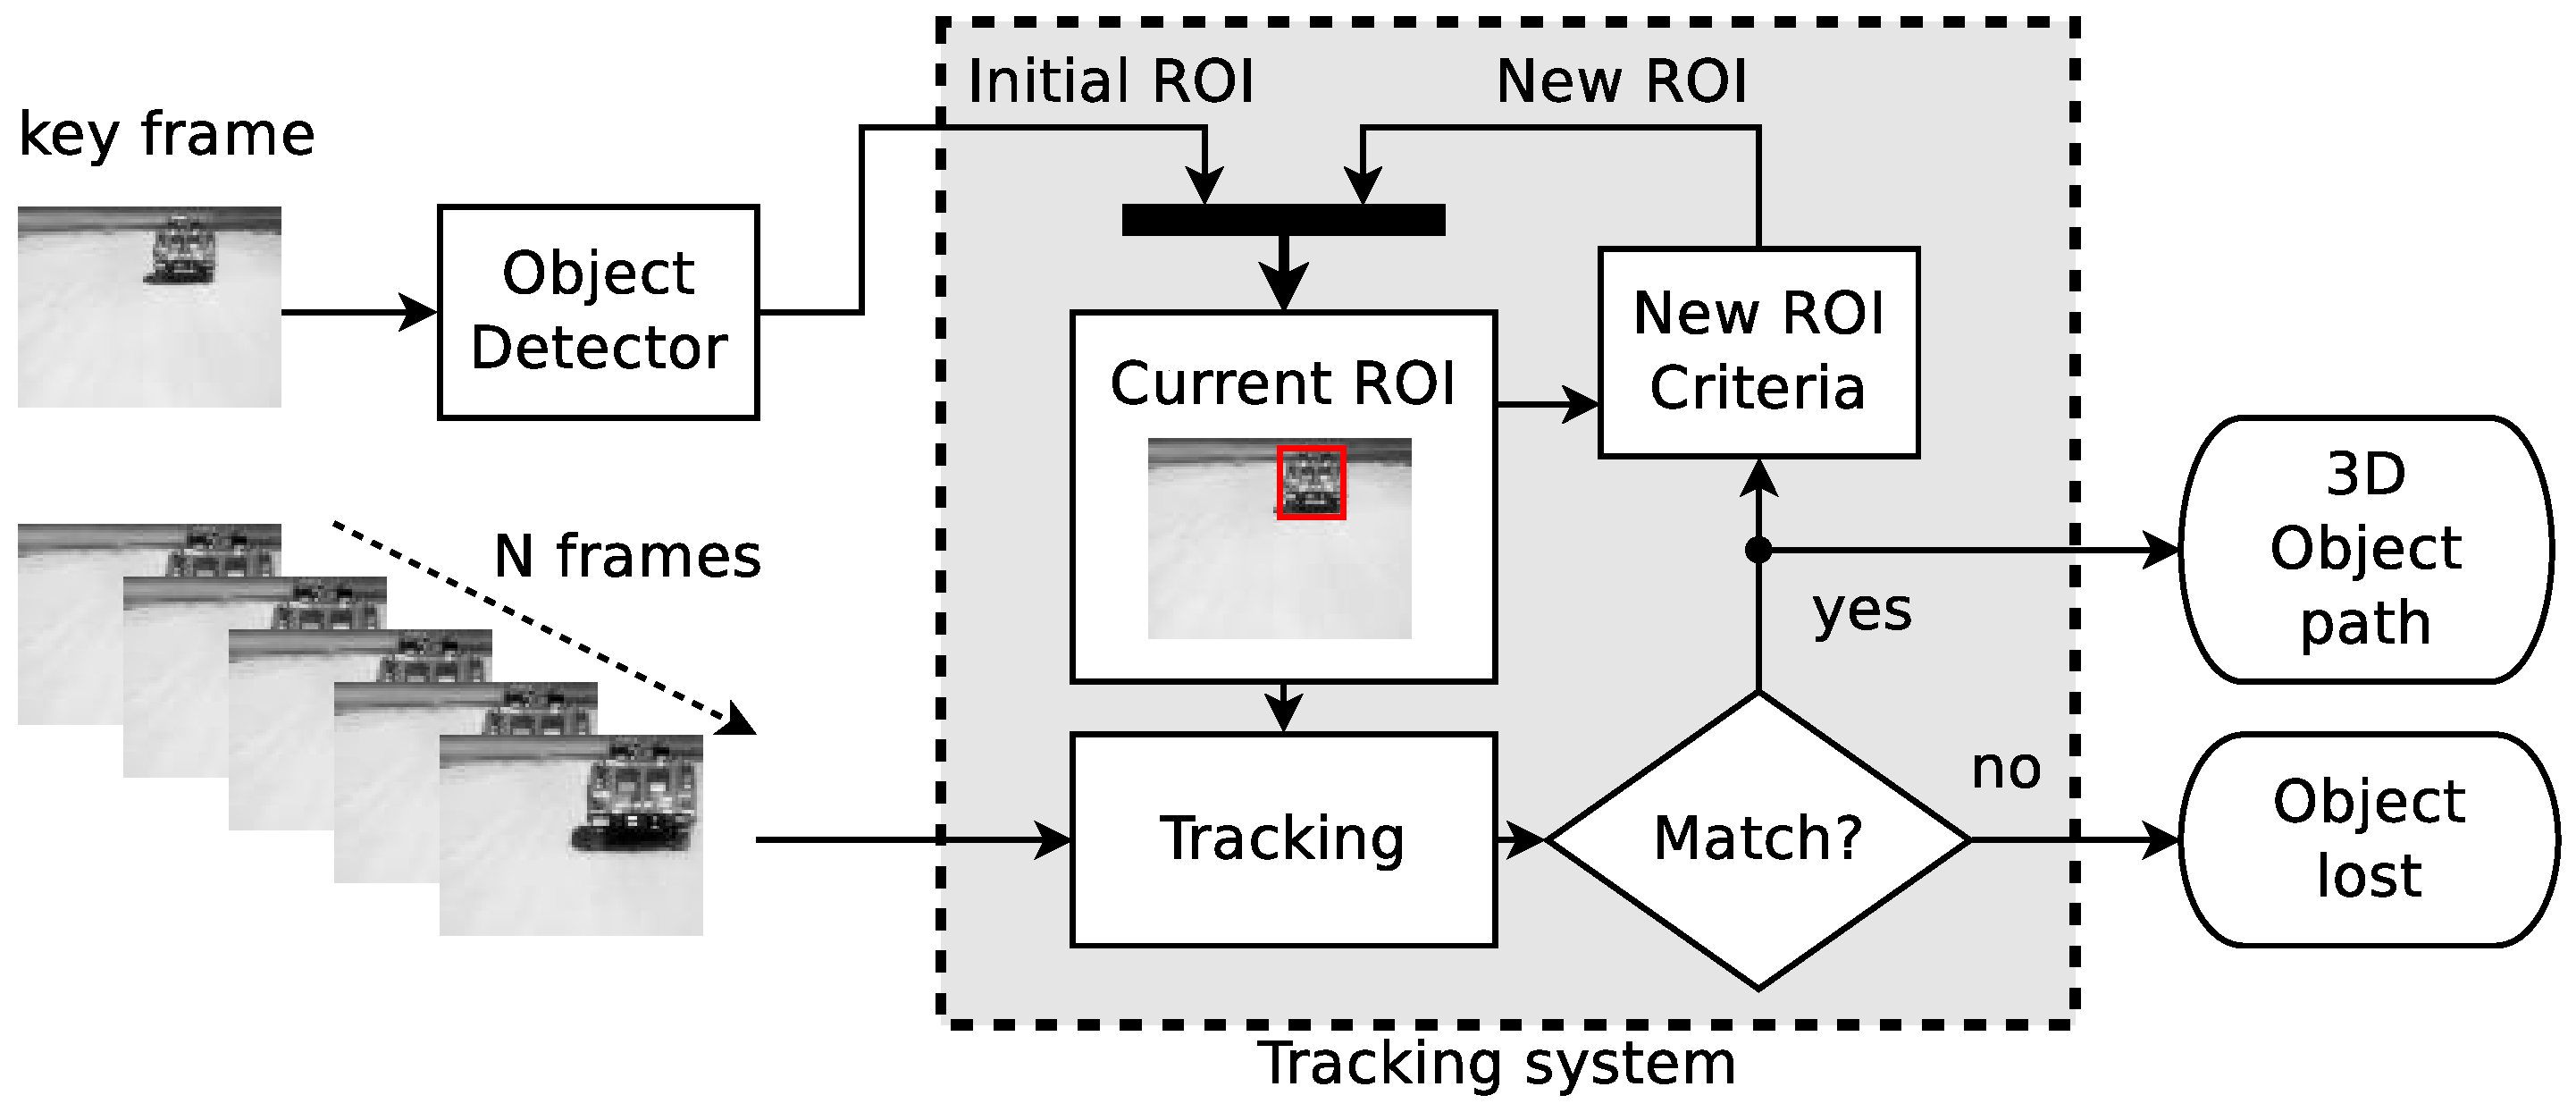
\includegraphics[width=\columnwidth]{images/figure1-diagram1.eps}
\caption{The target is identified from a highest value of correlation (CCP) between a selected ROI and an analysis region in
the $WOS$ of a current frame; the result of this process is a displacement which is  returned as vector field.}
\label{fig:system}
\end{figure}

\end{comment}
A proposta do algoritmo se baseia em um sistema de seguimento em três dimensões, que gera informações
da posição do objeto de interesse; com esta informação é calculada a velocidade,
sendo esta relativa ao observador.

O algoritmo ilustrado na Figura \ref{fig:system} tem como parâmetro inicial uma imagem com o
objeto de interesse, dentro de uma $ROI$; posteriormente, 
o sistema analisará as imagens subsequentes procurando regiões semelhantes à $ROI$
e salvará as posições do objeto de interesse em cada imagem.

\begin{figure}[h]
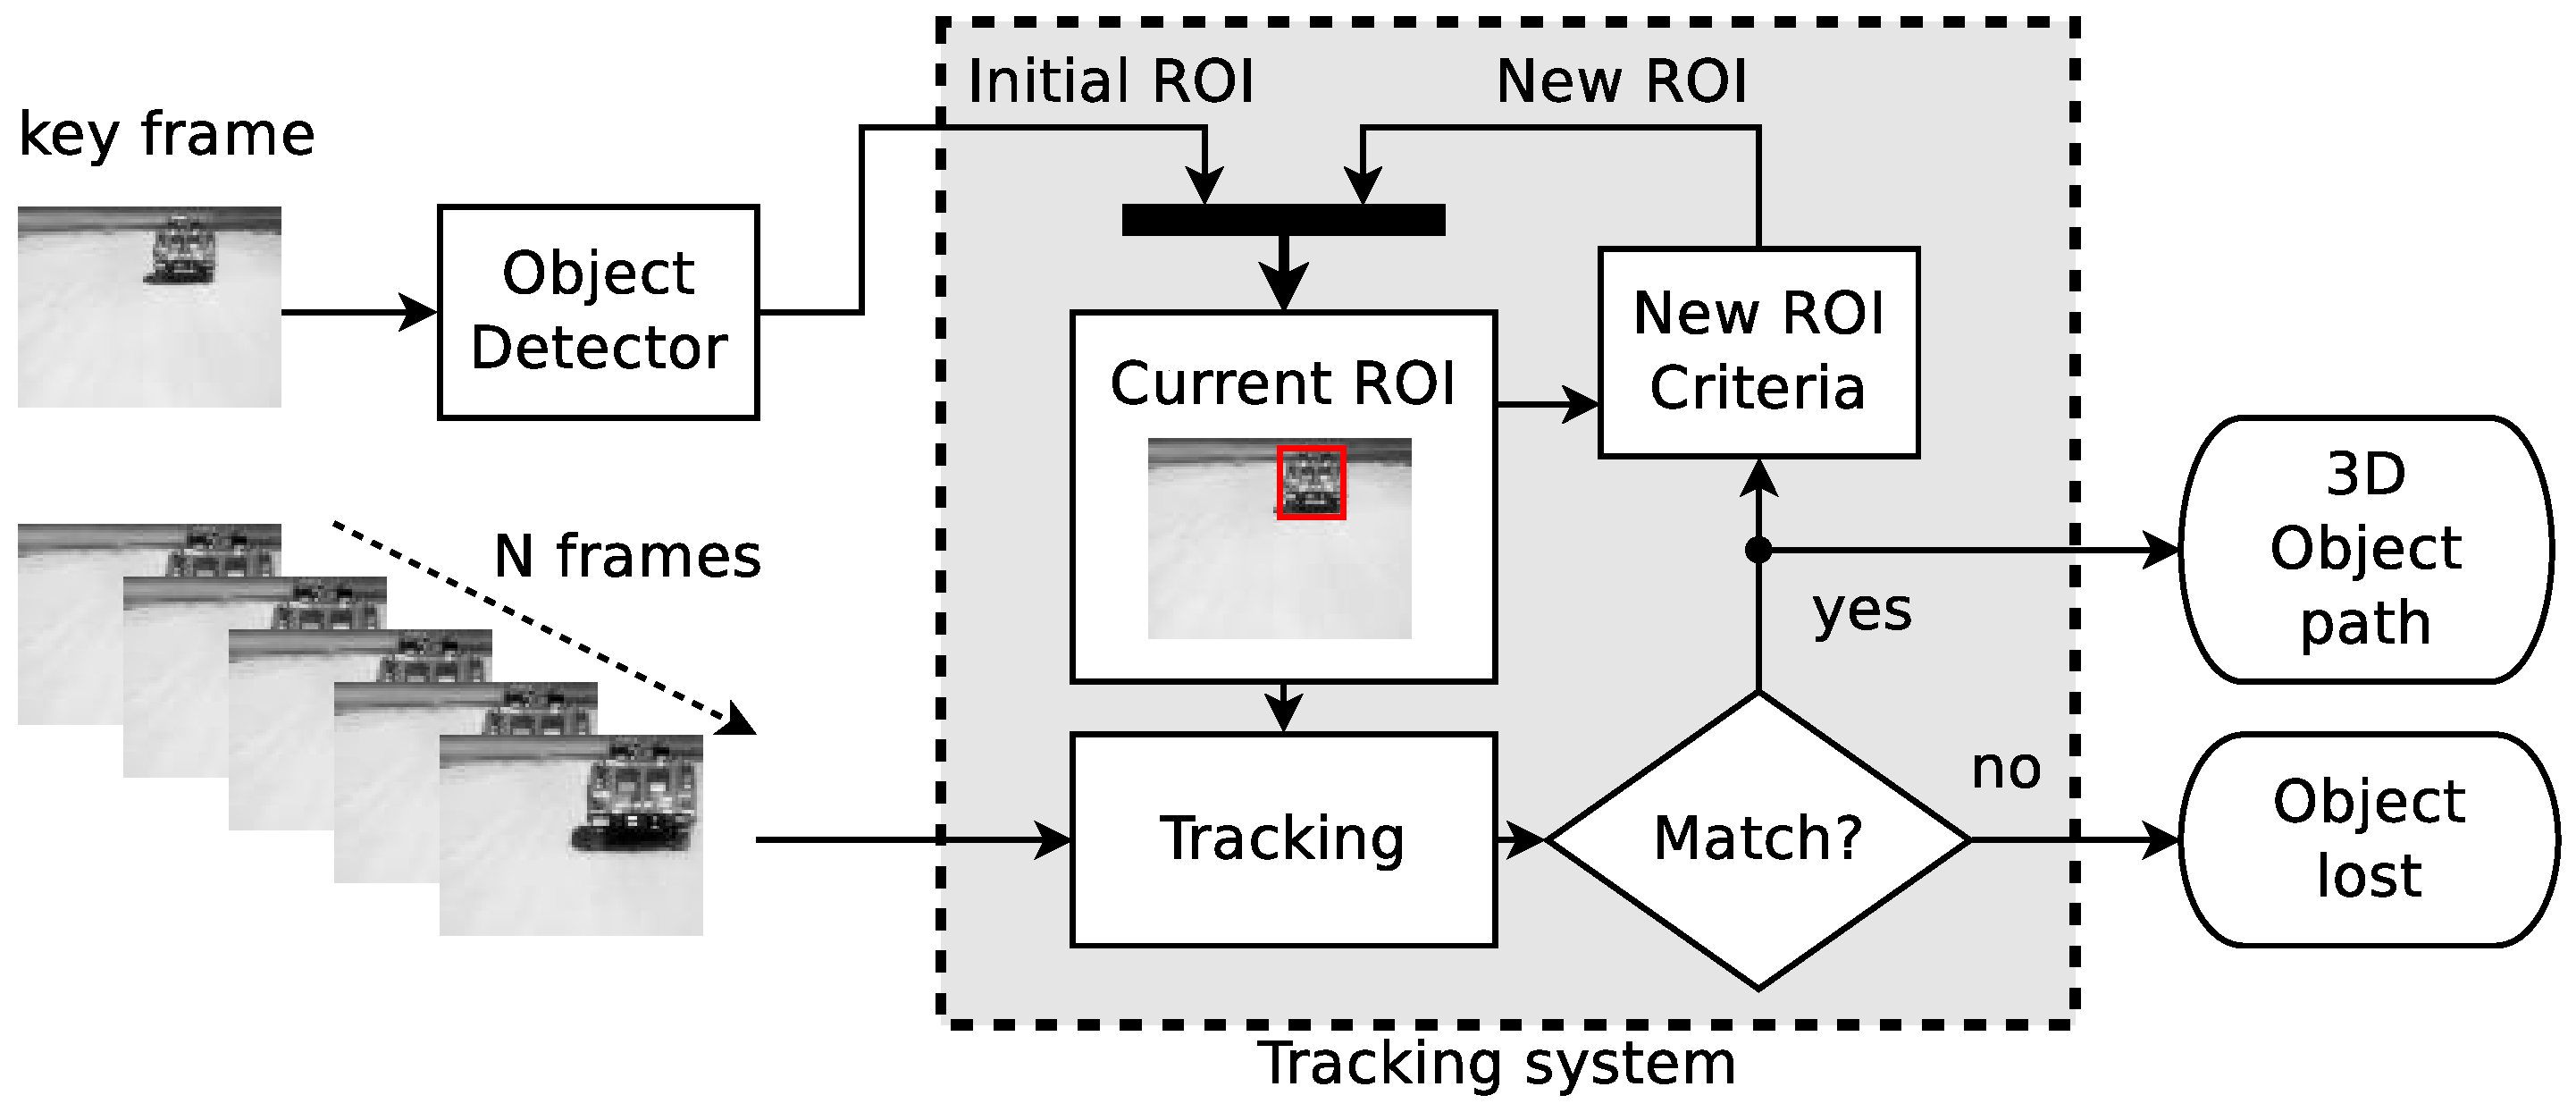
\includegraphics[width=\columnwidth]{images/figure1-diagram1.eps}
\caption{Proposta de algoritmo para rastreamento de objetos baseado no PIV}
\label{fig:system}
\end{figure}

\begin{comment}
In a two dimensional analysis, the tracked target given us information about its horizontal 
and vertical position and it is relative to the perpendicular velocity with respect to the observer.
When the target is analyzed in three dimensions, 
the initial $ROI$ has the position $(x=x_0,y=y_0,d=d_0=1)$;
where, $x_0$ and $y_0$ represent a position (horizontal and vertical) in the analyzed image,
and $d_0=1$ represents the initial depth position of target in the $ROI$ (normalized by definition to $1.0$).
Thus, all the results of depth will be relative to this value. In this sense, the relative velocity and 
the factor of approaching or departure can be calculated.

The Algorithm \ref{alg:system} shows a global vision of system described in the 
Fig. \ref{fig:system}, the functions ($multiscale\_match\_criterion$ and $renew\_roi\_criteria$) used in the algorithm 
will be explicated in the next sections. The algorithm receives as input parameters
A initial $ROI$, your position and a stream of $N$ images; with these data, the
algorithm returns a structure called $PATH$ with the position of target in each image frame,
being $PATH\{i\}=(x_i,y_i,d_i)$ the position of analysis region with target in the image $I_i$.
\end{comment}

A posição em pixels, do objeto de interesse na imagem, fornece informações 
sobre a posição horizontal e vertical relativa ao angulo de visão e 
distancia do observador; dando assim uma perspetiva 
da posição do objeto em 2D, $(x, y)$, sendo $x$ e $y$ as posições 
horizontal e vertical em pixels, respectivamente. Para analisar o objeto de interesse em 
3D, uma componente a mais é incluída, de modo que a posição do objeto esteja representada
por o ponto $(x, y, d)$, onde $d$ representa a profundidade 
do objeto na imagem (é dizer distancia entre o objeto e o observador), 
dado que para todos os cálculos o valor de profundidade
será expressado em função da posição inicial ($d_0$) do objeto de interesse na primeira imagem,
para fines práticos, este valor será normalizado a $d_0=1.0$.
A partir
deste valor, será possível mensurar a velocidade e um fator de aproximação $\beta$ do objeto
de forma relativa à posição inicial $d_0$; de modo que valores de $d=\beta d_0$
maiores que $1.0$ indicarão objetos mais distantes e valores menores que $1.0$, objetos mais próximos.

O algoritmo \ref{alg:system}, representa a sequência das 
ações descritas na Figura \ref{fig:system}. As funções 
 ($multiscale\_match\_criterion$ e $renew\_roi\_criteria$) serão discutidas na próxima seção. 
O algoritmo \ref{alg:system} recebe como entradas, a $ROI$ (que contem o objeto de interesse), 
a posição inicial $P_0=(x_0, y_0, d_0)$
da $ROI$   
e uma sequência de $N$ imagens. É importante notar que chamaremos $P_0$ à posição inicial
da $ROI$ na primeira imagem e $P_{ROI}=(x_{ROI}, y_{ROI}, d_{ROI})$ a posição atual da região
de interesse, dado que o algoritmo atualiza a $ROI$ quando por o deslocamento e perspetiva da imagem
o objeto cambia de forma; finalmente, o processo retorna 
uma estrutura chamada $PATH$ com a posição do objeto de interesse em cada imagem, sendo $PATH\{i\}=(x_i,y_i,d_i)$
a posição do objeto de interesse na imagem $I_i$.


\begin{comment}
\begin{algorithm}
 \KwData{An initial $ROI$, your position $P_0$ and a stream of images, $I_i$, for $0\leq i < N$. }
 \KwResult{$3D$ target $PATH$ or a target lost message. }
 $i \leftarrow 0$ \;
~\\
\While{$i < N$ }
{
    $\{AR,P,r\} \leftarrow multiscale\_match\_criterion(ROI,P_0,I_i)$\;
    
    $\{ROI,P_0,Found\} \leftarrow renew\_roi\_criteria(ROI,P_0,AR,P,r)$\;
    \eIf{Found}{
      $PATH\{i\}  \leftarrow P$\;
    }{
      break while loop\;
    }
}
~\\
\Return PATH \;
\caption{How to get a $3D$ target path.}
\label{alg:system}
\end{algorithm}
\end{comment}

\begin{algorithm}
 \KwData{$ROI$ e posição $P_0$ na primeira imagem, e uma sequência de imagens, $I_i$, para $0\leq i < N$. }
 \KwResult{A variável $PATH$ com a ruta do objeto em $3D$ ou uma mensagem de objeto perdido. }
 $i \leftarrow 0$ \;
 $P_{ROI} \leftarrow P_0$ \;
 $P \leftarrow P_0$ \;
~\\
\While{$i < N$ }
{
    $\{AR,P,r\} \leftarrow multiscale\_match\_criterion(ROI,P,I_i)$\;
    
    $\{ROI,P_{ROI},Found\} \leftarrow renew\_roi\_criteria(ROI,P_{ROI},AR,P,r)$\;
    \eIf{Found}{
      $PATH\{i\}  \leftarrow P$\;
    }{
      break while loop\;
    }
}
~\\
\Return PATH \;
\caption{Obtenção da trajetória em $3D$ do objeto de interesse.}
\label{alg:system}
\end{algorithm}

%Diagrama1
 %A gente vai explicar o algoritmo como uma caixa fechada , que coisa entra e que coisa sai
 %e os parametros a sintonizar.
 % como usar ele quando implementado, como se fosse uma caixa preta.
